% Title
%
% Examples
% 1. Send Receive entire View (1D and 2D)
%    - CUDA Aware
%    - Performance Consideration just on 1D
%      - Direct CudaSpace
%      - Direct CudaUVMSpace (accessing data before/after host/cuda)
%      - Writing from device to CudaPinnedHostSpace
%      - Explicit Copy to CudaPinnedHostSpace
%      - Explicit copy to CudaSpace
% 2. Strategy for buffers for all neighbors: 2D LayoutRight
%      - get consectuive subview for each neighbor, but fill in one go
% 3. Sparse Send (pack/unpack):
%      - using index list to fill
%      - using parallel_scan vs atomics to build an index list
%      - discuss latencies: launching kernels, MPI, fences, ...
% 4. Overlapping inner calculations with communication
%      - using streams, overlap force computation on particles which only have owned neighbors with communication
% 5. Mapping ranks to GPUs

\begin{frame}[fragile]

  {\Huge MPI - Kokkos Interoperability}

  \vspace{10pt}

  {\large Writing a hybrid MPI - Kokkos program.}

  \vspace{20pt}

  \textbf{Learning objectives:}
  \begin{itemize}
    \item {How to send data from Kokkos Views.}
    \item {How to overlap communication and computation.}
    \item {Buffer packing strategies.}
    \item {How to generate sparse index lists.}
  \end{itemize}

  \vspace{-20pt}

\end{frame}

%==========================================================================

\begin{frame}{MPI + Kokkos}
  \begin{center}
    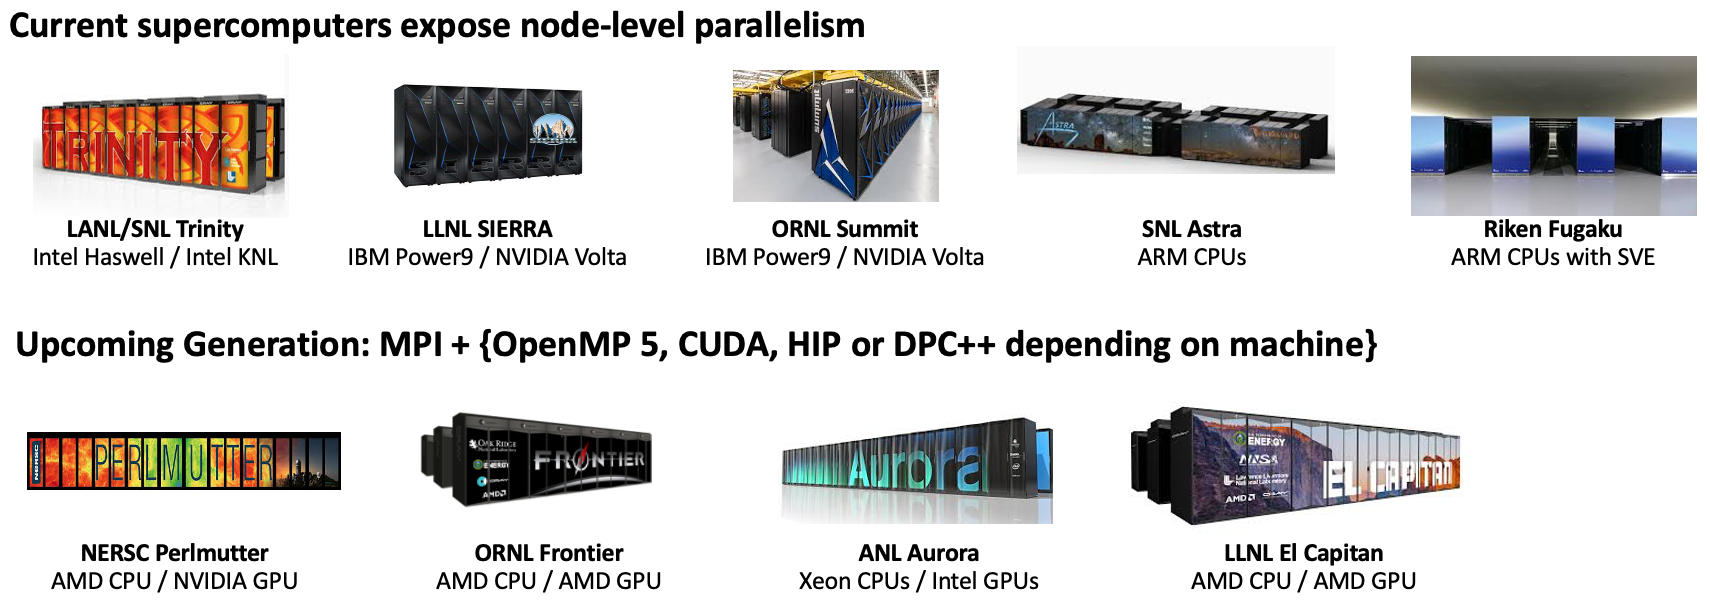
\includegraphics[width=1.05\textwidth]{figures/Architecture-Overview-MPI}
  \end{center}

\begin{itemize}
	\item Today supercomputers are clusters with disjoint address spaces
	\item One additional level of concurrency: node-level
	\item Allow MPI+Kokkos hybrid applications (using patterns, views, spaces, etc.)
\end{itemize}

\end{frame}

\begin{frame}[fragile]{MPI + Kokkos}
\textbf{Why mix MPI with Kokkos}
\begin{itemize}
  \item Need to address internode data transfers
  \item MPI is the de-facto standard
  \item MPI is well supported on all platforms
  \begin{itemize}
     \item MPI also knows how to talk to GPUs
  \end{itemize}
  \item The legacy code you want to port is already using MPI
  \item Programming explicitly to the parallelism hierarchy can help
\end{itemize}

\pause
\textbf{Are there any alternatives?}
\begin{itemize}
  \item You can potentially use PGAS models (discussed later).
  \item Global tasking models may work for you
  \begin{itemize}
    \item Kokkos has been used with Uintah for years
    \item LANL explores combining Legion and Kokkos with our support
  \end{itemize}
\end{itemize}
\end{frame}

\begin{frame}[fragile]{Motivating Example - Vector Shift}
  Simple Shifting of data:

  \begin{code}[keywords={View,double,int}]
  View<double*> A("A",N), B("B",N);
  // Single Device
  parallel_for("Shift",N,KOKKOS_LAMBDA(int i) {
    B((i+K)%N) = A(i);
  });
  \end{code}

\pause
  Lets assume we have R ranks:
  \begin{itemize}
    \item Now each rank owns N/R elements
    \item Rank j needs to send K elements to rank j+1
      \begin{itemize}
         \item j is sending the last K elements of A
      \end{itemize}
    \item Rank j needs to receive K elements from rank j-1
      \begin{itemize}
         \item j is receiving into the first K elements of B
      \end{itemize}
  \end{itemize}
\end{frame}

\begin{frame}[fragile]{Hybrid Programming 1}
\begin{itemize}
 \item The MPI Interface uses raw pointers
 \begin{lstlisting}
Kokkos::View<...> recv_view(...);
Kokkos::View<...> send_view(...);
void* recv_ptr = recv_view.data();
void* send_ptr = send_view.data();
  \end{lstlisting}
 \item Data needs to be stored contiguously $\Rightarrow$ \texttt{LayoutStride} not possible
 \item Data stored on the device requires GPU-aware MPI implementations. Otherwise, copying to the host is necessary
 \begin{lstlisting}
auto recv_view_h = Kokkos::create_mirror_view_and_copy(
  Kokkos::DefaultHostExecutionSpace{}, recv_view_d);
auto send_view_h = Kokkos::create_mirror_view_and_copy(
  Kokkos::DefaultHostExecutionSpace{}, send_view_d);
void* recv_ptr = recv_view_h.data();
void* send_ptr = send_view_h.data();
  \end{lstlisting}
\end{itemize}
\end{frame}

\begin{frame}[fragile]{Hybrid Programming 1}
Then the usual MPI functions can be used:

\vspace{10pt}
 \begin{code}[keywords={MPI_Request,MPI_Irecv,MPI_Isend,MPI_Waitall}]
MPI_Request requests[2];
MPI_Irecv(recv_ptr,recv_view.size(),MPI_DOUBLE,
          source,1,MPI_COMM_WORLD,&requests[0]);
// Send the buffer
MPI_Isend(send_ptr,send_view.size(),MPI_DOUBLE,
          target,1,MPI_COMM_WORLD,&requests[1]);
// Wait for communication to finish
MPI_Waitall(2,requests,MPI_STATUSES_IGNORE);
  \end{code}

\pause
\vspace{10pt}
In our example \texttt{send\_view} and \texttt{recv\_view} are just subviews:

\vspace{5pt}
\begin{code}[keywords={subview,make_pair,auto}]
auto send_view = Kokkos::subview(A,std::make_pair(myN-K, myN));
auto recv_view = Kokkos::subview(B,std::make_pair(0, K));
\end{code}
\end{frame}

\begin{frame}[fragile]{Simple Overlapping Communication}
  \textbf{Overlap communication with computation if possible!}

  \begin{itemize}
     \item Make sure compute kernel don not access send/recv buffers
     \item Post sends and recvs first
     \item Launch kernel
     \item Wait on MPI
  \end{itemize}

  \pause
  Vector-Shift Example:
\begin{code}[keywords={subview,MPI_Request,MPI_Irecv,MPI_Isend,parallel_for,MPI_Waitall}]
auto send_view = Kokkos::subview(A,std::make_pair(myN-K, myN));
auto recv_view = Kokkos::subview(B,std::make_pair(0, K));
MPI_Request requests[2];
// Post sends/recv
MPI_Irecv(recv_ptr,recv_view.size(),MPI_DOUBLE,
          source,1,MPI_COMM_WORLD,&requests[0]);
MPI_Isend(send_ptr,send_view.size(),MPI_DOUBLE,
          target,1,MPI_COMM_WORLD,&requests[1]);
parallel_for("ShiftA",RangePolicy<>(K,myN), 
  KOKKOS_LAMBDA(int i) { B(i) = A(i-K); });
// Wait for communication to finish
MPI_Waitall(2,requests,MPI_STATUSES_IGNORE);
\end{code}
\end{frame}


\begin{frame}[fragile]{Initializing MPI}
\textbf{Technical requirements}
\begin{itemize}
    \item Initialize MPI before Kokkos
    \begin{lstlisting}
int main(int argc, char* argv[]) {
  MPI_Init(&argc,&argv);
  Kokkos::initialize(argc,argv);
  [...]
  Kokkos::finalize();
  MPI_Finalize();
  }
    \end{lstlisting}
    \item By default, GPUs are distributed in a round-robin fashion if there are multiple.
	\item Use \texttt{mpicxx} as compiler
 	and \texttt{OMPI\_CXX=<path-to-kokkos-install>/nvcc\_wrapper} (for OpenMPI)
  	or use
\begin{texttt}find\_package(MPI REQUIRED)\end{texttt}
 with \texttt{CMake}.
\end{itemize}
\end{frame}


\begin{frame}[fragile]{Exercise: Send Data between MPI Processes}

  \begin{small}
  \begin{itemize}
  \item Location: \ExerciseDirectory{mpi\_pack\_unpack}
  \item Add missing MPI calls to \texttt{RunPackCommUnpackTest::run\_comm()}.
  \item Compile and run on CPU, and then on GPU.
  \end{itemize}
  \end{small}

\begin{code}
mkdir build && cd build
export Kokkos_DIR=<path-to-kokkos-install>
cmake .. && make
# Run exercise
mpiexec -np 2 MPIPackUnpack
\end{code}

Command line arguments
%   \begin{scriptsize}
  \begin{itemize}
  \item Vary size of data
  \item Vary size of buffers
  \item Number of repeats for timing
  \item Copy to host first
  \end{itemize}
%   \end{scriptsize}
\end{frame}

\begin{frame}[fragile]{Explicit Message Buffers}
\textbf{Sometimes extra send/recv buffers are needed}
\begin{itemize}
  \item Buffer data which is getting written to again
  \item Sparse data needs to be sent or received
    \begin{itemize}
       \item In particular if isn't regular strided
       \item Will discuss some best practices later
    \end{itemize}
  \item The system doesn't allow MPI to access some memory space
\end{itemize}

\pause
\textbf{The Pack-Send/Recv-Unpack Cycle:}
\begin{itemize}
  \item Post Irecvs
  \item Pack buffers
  \item Post Isends
  \item Wait on message completion
  \item Unpack buffers
\end{itemize}
\end{frame}

\begin{frame}[fragile]{Explicit Message Buffers}
Based on our Kokkos knowledge of Execution and Memory Spaces the following question arises:

\textbf{Where should the pack kernel run, and where should it pack to?}

\begin{itemize}
  \item Run the pack kernel wherever the data lives.
  \item The best memory space for the pack buffer depends.
  \item Sometimes packing into a device buffer, and still explicitly copying to the host is best.
\end{itemize}

\textit{There are a number of options for CUDA for example:}

\vspace{5pt}
\begin{tabular}{l|l|l}
\textbf{Data Space} & \textbf{Pack Buffer Space} & \textbf{Explicit HostCopy} \\ \hline
CudaSpace & CudaSpace & yes \\
CudaSpace & CudaSpace & no \\
CudaSpace & CudaUVMSpace & no \\
CudaSpace & CudaHostPinnedSpace & no \\
\end{tabular}

\end{frame}

\begin{frame}[fragile]{Performance Results}

\textbf{CudaSpace vs CudaUVMSpace vs CudaHostPinnedSpace}
\begin{itemize}
\item Time relative to CudaSpace on single socket (lower is better).
\item Performance is very sensitive to system and configurations!!
\end{itemize}

\pause
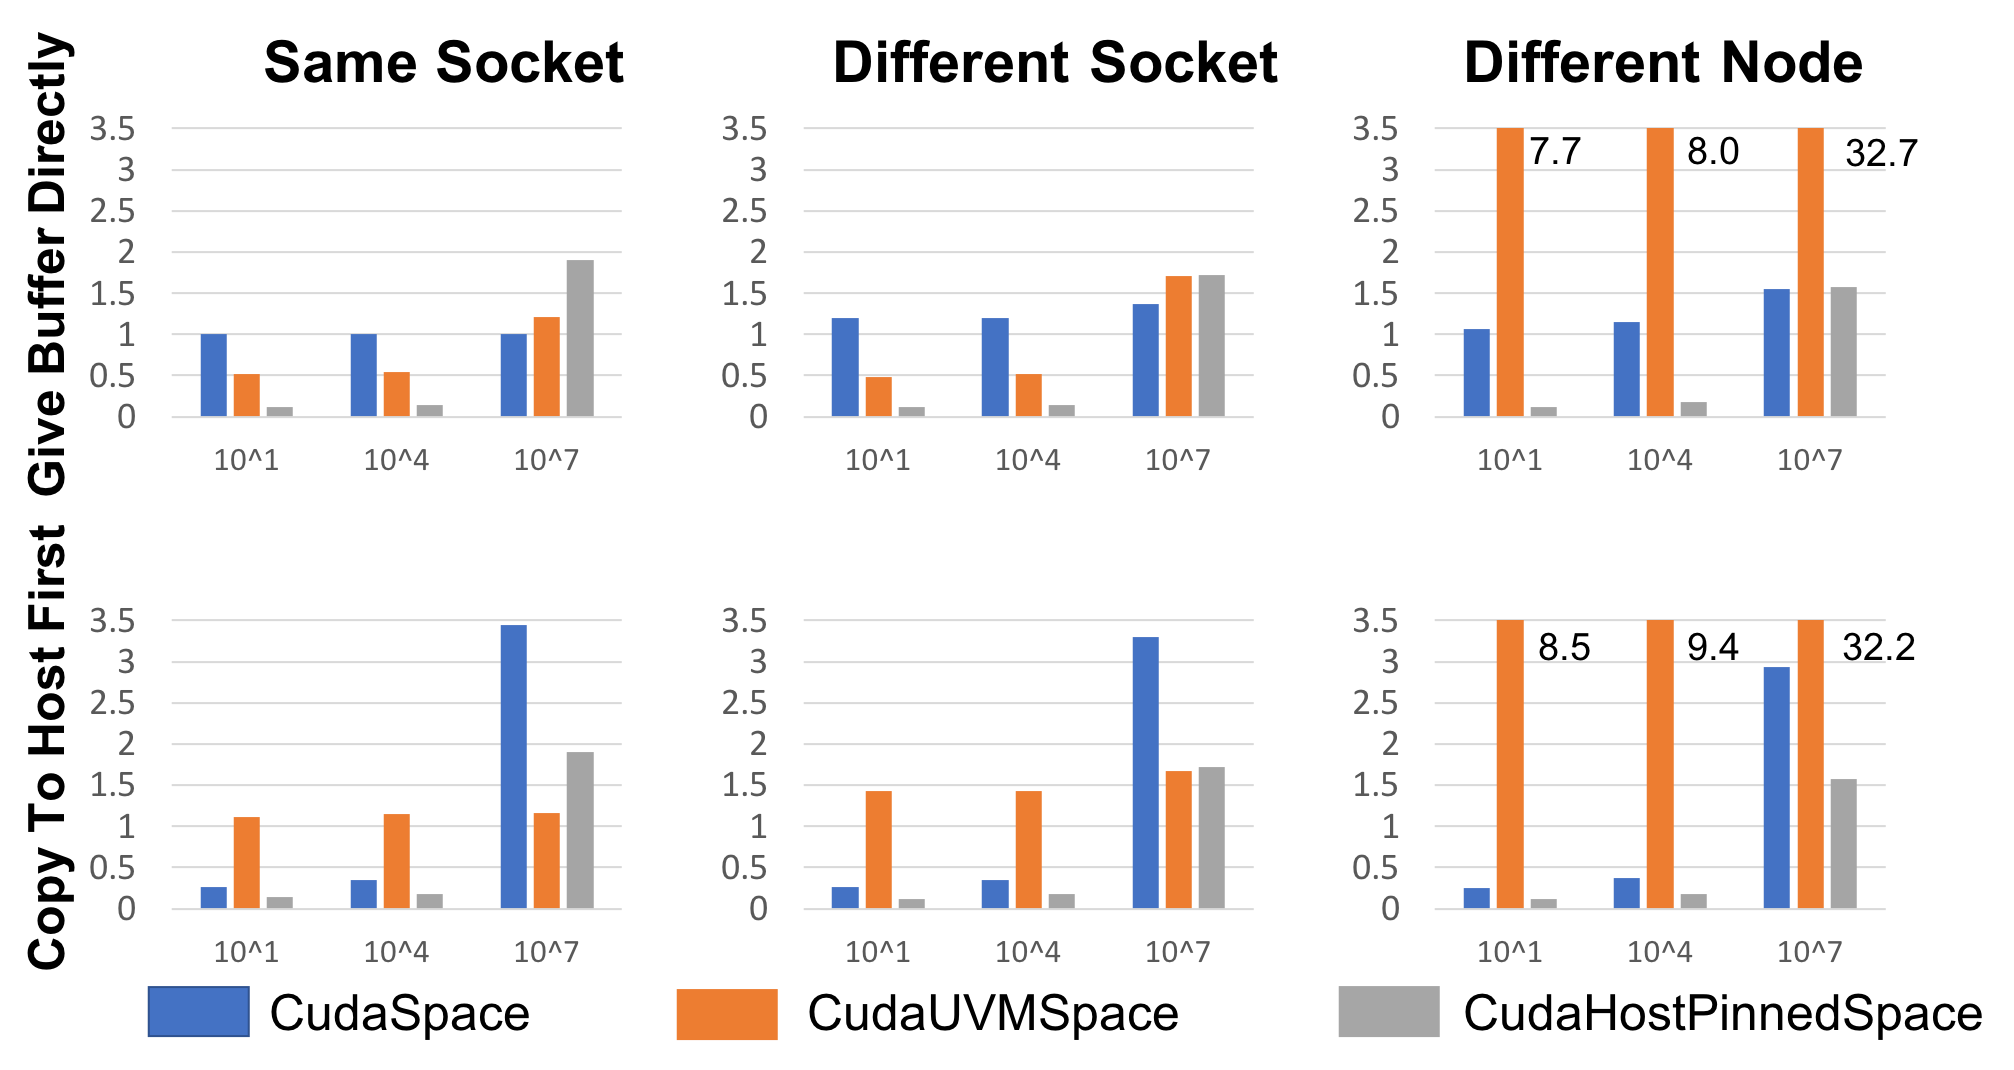
\includegraphics[width=\textwidth]{figures/MPI-Performance}
\end{frame}

\begin{comment}
\begin{frame}[fragile]{Performance Results Exercise}
Excluding parallel\_fors, copy to host
     \pgfplotstableread{
 size      Cuda       CudaHostPinnedh CudaUVM   Host
 10        0.0000533  0.0000171       0.0003804 0.0000178
 100       0.0000541  0.0000174       0.0003738 0.0000178
 1000      0.0000584  0.0000180       0.0003736 0.0000191
 10000     0.0000797  0.0000228       0.0003794 0.0000238
 100000    0.0002245  0.0000468       0.0003948 0.0000478
 1000000   0.0020995  0.0005860       0.0006549 0.0005916
 10000000  0.0191008  0.0065910       0.0035631 0.0066248
 100000000 0.1940944  0.0663647       0.0347974 0.0656929
}\tablecompareperformance

\begin{figure}
\centering
\begin{tikzpicture}[scale=0.9]
    \begin{loglogaxis}[
      legend style={legend pos=north west},
      xlabel={N},
      ylabel={time in (s)},
      ymin=1e-5,
      ymax=1,
      grid, thick
    ]
      \addplot table[x expr={\thisrowno{0}}, y index={1}] {\tablecompareperformance};
      \addlegendentry{Cuda}
      \addplot table[x expr={\thisrowno{0}}, y index={2}] {\tablecompareperformance};
      \addlegendentry{CudaHostPinned}
      \addplot table[x expr={\thisrowno{0}}, y index={3}] {\tablecompareperformance};
      \addlegendentry{CudaUVM}
      \addplot table[x expr={\thisrowno{0}}, y index={4}] {\tablecompareperformance};
      \addlegendentry{Host}
      \end{loglogaxis}
    \end{tikzpicture}
\end{figure}
\end{frame}

\begin{frame}[fragile]{Performance Results Exercise}
Excluding parallel\_fors, don't copy to host
     \pgfplotstableread{
 size      Cuda       CudaHostPinnedh CudaUVM   Host
 10        0.00033222 0.00001230      0.00011110 0.00001225
 100       0.00033221 0.00001281      0.00011025 0.00001258
 1000      0.00033359 0.00001356      0.00011182 0.00001417
 10000     0.00033872 0.00001800      0.00011358 0.00001819
 100000    0.00035633 0.00004147      0.00013237 0.00004257
 1000000   0.00053719 0.00053546      0.00042869 0.00051637
 10000000  0.00216941 0.00659140      0.00388138 0.00657494
 100000000 0.01844423 0.06551141      0.03870359 0.06524309
}\tablecompareperformancegpuaware

\begin{figure}
\centering
\begin{tikzpicture}[scale=0.9]
    \begin{loglogaxis}[
      legend style={legend pos=north west},
      xlabel={N},
      ylabel={time in (s)},
      ymin=1e-5,
      ymax=1,
      grid, thick
    ]
      \addplot table[x expr={\thisrowno{0}}, y index={1}] {\tablecompareperformancegpuaware};
      \addlegendentry{Cuda}
      \addplot table[x expr={\thisrowno{0}}, y index={2}] {\tablecompareperformancegpuaware};
      \addlegendentry{CudaHostPinned}
      \addplot table[x expr={\thisrowno{0}}, y index={3}] {\tablecompareperformancegpuaware};
      \addlegendentry{CudaUVM}
      \addplot table[x expr={\thisrowno{0}}, y index={4}] {\tablecompareperformancegpuaware};
      \addlegendentry{Host}
      \end{loglogaxis}
    \end{tikzpicture}
\end{figure}
\end{frame}

\begin{frame}[fragile]{Performance Results Exercise}
different sockets
     \pgfplotstableread{
 size      Cuda       CudaHostPinnedh CudaUVM    Host
 10        0.041782   0.003966        0.017534   0.001408
 10000     0.041473   0.005486        0.018058   0.027909
 10000000  1.232990   1.551578        1.534636   72.761595
}\tablecompareperformancefull

\begin{figure}
\centering
\begin{tikzpicture}[scale=0.9]
    \begin{loglogaxis}[
      legend style={legend pos=north west},
      xlabel={N},
      ylabel={time in (s)},
      ymin=1e-3,
      ymax=100,
      grid, thick
    ]
      \addplot table[x expr={\thisrowno{0}}, y index={1}] {\tablecompareperformancefull};
      \addlegendentry{Cuda}
      \addplot table[x expr={\thisrowno{0}}, y index={2}] {\tablecompareperformancefull};
      \addlegendentry{CudaHostPinned}
      \addplot table[x expr={\thisrowno{0}}, y index={3}] {\tablecompareperformancefull};
      \addlegendentry{CudaUVM}
      \addplot table[x expr={\thisrowno{0}}, y index={4}] {\tablecompareperformancefull};
      \addlegendentry{Host}
      \end{loglogaxis}
    \end{tikzpicture}
\end{figure}
\end{frame}

\begin{frame}[fragile]{Performance Results Exercise}
different sockets, copy to host
     \pgfplotstableread{
 size      Cuda       CudaHostPinnedh CudaUVM    Host
 10        0.008601   0.004460        0.046049   0.001922
 10000     0.012437   0.005989        0.049750   0.028535
 10000000  2.969337   1.551063        1.505497   71.818246
}\tablecompareperformancefullhost

\begin{figure}
\centering
\begin{tikzpicture}[scale=0.9]
    \begin{loglogaxis}[
      legend style={legend pos=north west},
      xlabel={N},
      ylabel={time in (s)},
      ymin=1e-3,
      ymax=100,
      grid, thick
    ]
      \addplot table[x expr={\thisrowno{0}}, y index={1}] {\tablecompareperformancefullhost};
      \addlegendentry{Cuda}
      \addplot table[x expr={\thisrowno{0}}, y index={2}] {\tablecompareperformancefullhost};
      \addlegendentry{CudaHostPinned}
      \addplot table[x expr={\thisrowno{0}}, y index={3}] {\tablecompareperformancefullhost};
      \addlegendentry{CudaUVM}
      \addplot table[x expr={\thisrowno{0}}, y index={4}] {\tablecompareperformancefullhost};
      \addlegendentry{Host}
      \end{loglogaxis}
    \end{tikzpicture}
\end{figure}
\end{frame}

\begin{frame}[fragile]{Performance Results Exercise}
same sockets
     \pgfplotstableread{
 size      Cuda       CudaHostPinnedh CudaUVM    Host
 10        0.035284   0.004108        0.018218   0.001452
 10000     0.035542   0.005595        0.018763   0.033356
 10000000  0.900193   1.708386        1.087862   87.032740
}\tablecompareperformancefullsocket

\begin{figure}
\centering
\begin{tikzpicture}[scale=0.9]
    \begin{loglogaxis}[
      legend style={legend pos=north west},
      xlabel={N},
      ylabel={time in (s)},
      ymin=1e-3,
      ymax=100,
      grid, thick
    ]
      \addplot table[x expr={\thisrowno{0}}, y index={1}] {\tablecompareperformancefullsocket};
      \addlegendentry{Cuda}
      \addplot table[x expr={\thisrowno{0}}, y index={2}] {\tablecompareperformancefullsocket};
      \addlegendentry{CudaHostPinned}
      \addplot table[x expr={\thisrowno{0}}, y index={3}] {\tablecompareperformancefullsocket};
      \addlegendentry{CudaUVM}
      \addplot table[x expr={\thisrowno{0}}, y index={4}] {\tablecompareperformancefullsocket};
      \addlegendentry{Host}
      \end{loglogaxis}
    \end{tikzpicture}
\end{figure}
\end{frame}

\begin{frame}[fragile]{Performance Results Exercise}
same sockets, copy to host
     \pgfplotstableread{
 size      Cuda       CudaHostPinnedh CudaUVM    Host
 10        0.009128   0.004699        0.039293   0.002084
 10000     0.012310   0.006289        0.040151   0.028537
 10000000  3.799518   1.708801        1.036396   85.849318
}\tablecompareperformancefullhostsocket

\begin{figure}
\centering
\begin{tikzpicture}[scale=0.9]
    \begin{loglogaxis}[
      legend style={legend pos=north west},
      xlabel={N},
      ylabel={time in (s)},
      ymin=1e-3,
      ymax=100,
      grid, thick
    ]
      \addplot table[x expr={\thisrowno{0}}, y index={1}] {\tablecompareperformancefullhostsocket};
      \addlegendentry{Cuda}
      \addplot table[x expr={\thisrowno{0}}, y index={2}] {\tablecompareperformancefullhostsocket};
      \addlegendentry{CudaHostPinned}
      \addplot table[x expr={\thisrowno{0}}, y index={3}] {\tablecompareperformancefullhostsocket};
      \addlegendentry{CudaUVM}
      \addplot table[x expr={\thisrowno{0}}, y index={4}] {\tablecompareperformancefullhostsocket};
      \addlegendentry{Host}
      \end{loglogaxis}
    \end{tikzpicture}
\end{figure}
\end{frame}

\begin{frame}[fragile]{Performance Results Exercise}
different node
     \pgfplotstableread{
 size      Cuda       CudaHostPinnedh CudaUVM    Host
 10        0.036866   0.003910        0.270404   0.001427
 10000     0.039647   0.006262        0.283026   0.029009
 10000000  1.396050   1.415000        29.371574  73.402895
}\tablecompareperformancefullnode

\begin{figure}
\centering
\begin{tikzpicture}[scale=0.9]
    \begin{loglogaxis}[
      legend style={legend pos=north west},
      xlabel={N},
      ylabel={time in (s)},
      ymin=1e-3,
      ymax=100,
      grid, thick
    ]
      \addplot table[x expr={\thisrowno{0}}, y index={1}] {\tablecompareperformancefullnode};
      \addlegendentry{Cuda}
      \addplot table[x expr={\thisrowno{0}}, y index={2}] {\tablecompareperformancefullnode};
      \addlegendentry{CudaHostPinned}
      \addplot table[x expr={\thisrowno{0}}, y index={3}] {\tablecompareperformancefullnode};
      \addlegendentry{CudaUVM}
      \addplot table[x expr={\thisrowno{0}}, y index={4}] {\tablecompareperformancefullnode};
      \addlegendentry{Host}
      \end{loglogaxis}
    \end{tikzpicture}
\end{figure}
\end{frame}

\begin{frame}[fragile]{Performance Results Exercise}
different node, copy to host
     \pgfplotstableread{
 size      Cuda       CudaHostPinnedh CudaUVM    Host
 10        0.008674   0.004455        0.298826   0.001864
 10000     0.013019   0.006524        0.330559   0.040083
 10000000  2.640824   1.422987        29.231414  73.752908
}\tablecompareperformancefullhostnode

\begin{figure}
\centering
\begin{tikzpicture}[scale=0.9]
    \begin{loglogaxis}[
      legend style={legend pos=north west},
      xlabel={N},
      ylabel={time in (s)},
      ymin=1e-3,
      ymax=100,
      grid, thick
    ]
      \addplot table[x expr={\thisrowno{0}}, y index={1}] {\tablecompareperformancefullhostnode};
      \addlegendentry{Cuda}
      \addplot table[x expr={\thisrowno{0}}, y index={2}] {\tablecompareperformancefullhostnode};
      \addlegendentry{CudaHostPinned}
      \addplot table[x expr={\thisrowno{0}}, y index={3}] {\tablecompareperformancefullhostnode};
      \addlegendentry{CudaUVM}
      \addplot table[x expr={\thisrowno{0}}, y index={4}] {\tablecompareperformancefullhostnode};
      \addlegendentry{Host}
      \end{loglogaxis}
    \end{tikzpicture}
\end{figure}
\end{frame}
\end{comment}

\begin{frame}[fragile]{Explicit Message Buffers}
\textbf{Leveraging streams allow calculations and communication with explicit buffers to overlap!}
\begin{itemize}
  \item Execute packing, unpacking and deep\_copies with different streams than interior kernels.
  \item Submission order is important though
  \begin{itemize}
     \item Worksets are largely worked on in submission order even with CUDA streams
     \item Need to submit pack kernels first, then interiors kernel
     \item Unless priority streams are a thing ...
  \end{itemize}
  \item Fence the pack execution space instances only before issuing sends
  \item ExecutionSpace instances, and buffers need to be persistent - allocations add fencing
\end{itemize}
\end{frame}

\begin{frame}[fragile]{Explicit Message Buffers}
\textbf{Code Skeleton:}
\begin{code}[keywords={MPI_Irecv,parallel_for,fence,MPI_Isend,MPI_Waitall}]
  // Create execution space instances
  ExecSpace exec_pack(..), exec_comp(..);
  using exec_policy = RangePolicy<ExecSpace>;
  // Post Receives
  MPI_Irecv(...);
  // Launch pack kernel in pack exec instance
  // Likely this uses only few cores
  parallel_for("PackBuffer",
    exec_policy(exec_pack,0,N),fpack);
  // Launch compute kernel independent of message exchange
  parallel_for("Interior",
    exec_policy(exec_comp,0,N),finterior);
  // Wait for pack kernel to finish before sending data
  exec_pack.fence();
  MPI_Isend(...);
  // Wait for communication to finish
  MPI_Waitall(...);
  // Unpack received data - may still overlap with "Interior"
  parallel_for("UnpackBuffer",
    exec_policy(exec_pack,0,N),funpack);
  // Wait for all work to finish
  Kokkos::fence();
\end{code}

\end{frame}

\begin{frame}{Motivating Example - Heat Equation}
\textbf{3D Heat Conduction}
\begin{itemize}
\item Heat conduction inside the body
\item Thermal radiation (Black Body) on surface
\item Incoming power flow from one direction
\end{itemize}

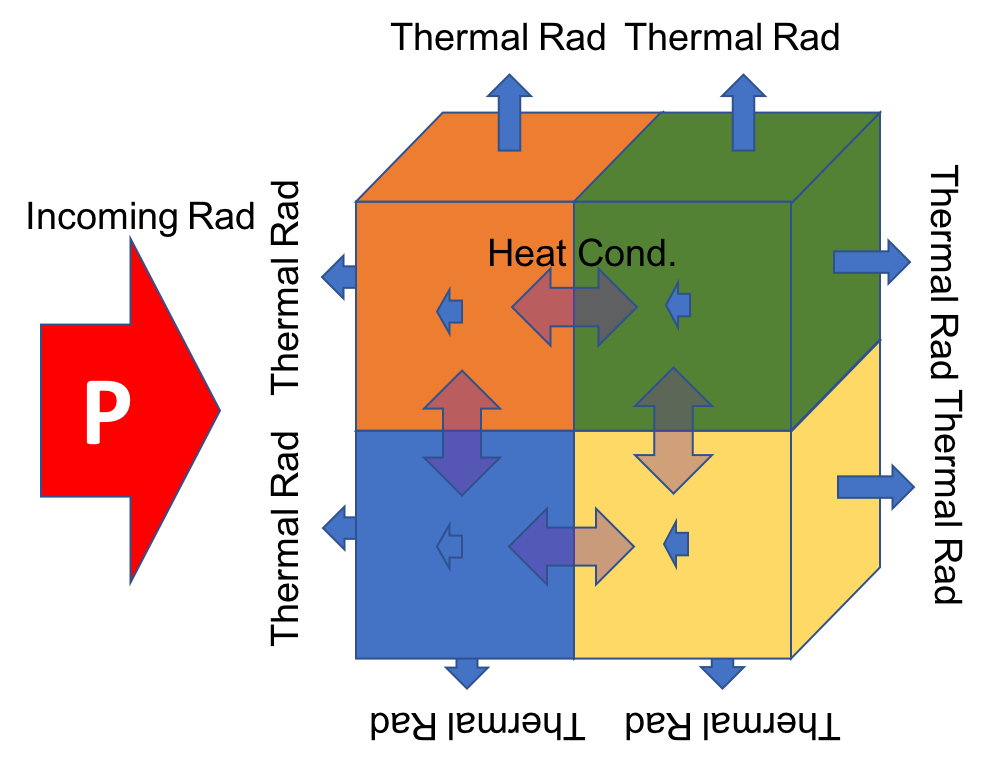
\includegraphics[width=0.65\textwidth]{figures/3DHeat}
\end{frame}

\begin{comment}
\begin{frame}{Motivating Example - Heat Equation}
Models distribution of heat given a heat source/sink $f$ over time
    \begin{align*}
       \partial_t u - \alpha \Delta_x u = f
    \end{align*}
    Using explicit Euler for time discretization gives
    \begin{align*}
       u^{n+1} = u^n + \Delta t (\alpha \Delta_x u^n + f(t_n))
    \end{align*}
    Finite difference discretization using central differences
    \begin{align*}
          u_{ijk}^{n+1} =& u_{ijk}^n + \Delta t f(t_n) \\
                         &+\frac{\Delta t}{h^2}\alpha (u_{i-1,j,k}^n -2 u_{i,j,k}^n + u_{i+1,j,k}^n \\
                         &\qquad\qquad+ u_{i,j-1,k}^n -2 u_{i,j,k}^n + u_{i,j+1,k}^n \\
                         &\qquad\qquad+ u_{i,j,k-1}^n -2 u_{i,j,k}^n + u_{i,j,k+1}^n)
    \end{align*}
\end{frame}

\begin{frame}{Motivating Example - Heat Equation}
Discretization
    \begin{align*}
          u_{ijk}^{n+1} =& u_{ijk}^n + \Delta t f(t_n) \\
                         &+\frac{\Delta t}{h^2}\alpha (u_{i-1,j,k}^n -2 u_{i,j,k}^n + u_{i+1,j,k}^n \\
                         &\qquad\qquad+ u_{i,j-1,k}^n -2 u_{i,j,k}^n + u_{i,j+1,k}^n \\
                         &\qquad\qquad+ u_{i,j,k-1}^n -2 u_{i,j,k}^n + u_{i,j,k+1}^n)
    \end{align*}
    \begin{itemize}
    \item Updating $u_{ijk}$ requires information for all the (direct) neighbors.
    \item Splitting the computational domain across multiple processes requires exchange of data $\Rightarrow$ MPI
    \end{itemize}

\end{frame}

\begin{frame}{Example - 3D Heat Equations}
  \textbf{Heat Source / Sink defined through the boundary conditions}
   \begin{itemize}
      \item Using surface black body thermal radiation as heat sink
      \begin{itemize}
        \item Using A as surface area of an element (its zero for all bulk elements)
      \end{itemize}
      \item Using a constant power density as heat source on one surface
      \begin{itemize}
        \item Turn the power of mid run.
        \item Use Ax as surface area exposed to the heat source
      \end{itemize}
   \end{itemize}
   \begin{align*}
      f(t_n) = -A_{ijk}*sigma*u^4 + Ax_{ijk}*P(t_n)
   \end{align*}
\end{frame}
\end{comment}

\begin{frame}{Simple Approach}
   \textbf{No Overlapping}

Data Structures:
\begin{itemize}
  \item T(x,y,z): temperature in cell (x,y,z)
  \item dT(x,y,z): temperature change in time increment dt
  \item T\_{left,right,up,down,front,back}: recv buffers for boundaries
  \item T\_{left\_out,...}: send buffers for boundaries
\end{itemize}

Time approach:
\begin{itemize}
  \item deep\_copy boundary layers as needed to contiguous send buffers
  \item Post MPI send/recv with send/recv buffers
  \item Launch kernel for interior elements doing heat conduction only
  \item Wait for MPI
  \item Compute updates for boundary elements using the recv buffers
\end{itemize}
\end{frame}

\begin{frame}{Optimized Pattern}
\textbf{Overlapping packing/unpacking with interior compute}

Getting better performance can be achieved by staging calls correctly, and using execution space instances:

\begin{itemize}
  \item Use 7 instances: interior, 6x boundary (left, right, ...)
  \item Issue Irecv
  \item Run up to 6 pack kernels using different exec space instances
  \item Launch interior kernel into its own instance
  \item Fence first boundary pack instance, issue Isend
  \item Fence other boundary packs and issue Isends one by one
  \item Wait for MPI operations to finish
  \item Issue boundary temperature update kernel
  \item Fence everything
\end{itemize}
\end{frame}

\begin{frame}[fragile]{Exercise: Optimize 3D Heat}
Optimize the basic MPI implementation of the 3D heat conduction code for GPU systems.

  \vspace{10pt}

  \textbf{Details}:
  \begin{small}
  \begin{itemize}
\item Location: \ExerciseDirectory{mpi\_heat\_conduction}
\item Use Execution Space instances for more overlapping
\item Order operations for maximum overlapping
\item Run with correct GPU mapping
\end{itemize}
  \end{small}

\ul{\textbf{Things to try:}}
  \begin{small}
  \begin{itemize}
  \item Try strong vs weak scaling
  \item Change Problem Size -X , -Y , -Z
  \item Play with buffer memory space
  \item Compare same socket, vs different socket, vs multi node perf
  \end{itemize}
  \end{small}
\end{frame}

\begin{frame}[fragile]{Sparse Data to be Send}
In the heat conduction example some surfaces were sparse, but regular.

\pause
\vspace{10pt}
\textbf{How best to generate index lists if data is not regular sparse?}

\pause
\vspace{10pt}
Example problems:
\begin{itemize}
  \item Send all particles which crossed the boundary.
  \item Send all elements in contact with the surface.
\end{itemize}

\pause
Use indirect pack kernel:
\begin{code}[keywords={parallel_for,send_list}]
  parallel_for("Pack",num_send, KOKKOS_LAMBDA(int e) {
    pack(e) = data(send_list(e));
  });
\end{code}

\pause
\textbf{How to generate the send\_list?}

\pause
$=>$ Use a \texttt{parallel\_scan}

\end{frame}


\begin{frame}[fragile]{Generating Index}

\textbf{Generating Index Lists via \texttt{parallel\_scan}}

\vspace{10pt}
\begin{itemize}
  \item \texttt{bool needs\_send(int e)} is true if element \texttt{e} needs to be sent:
\end{itemize}

\begin{code}[keywords={parallel_scan,send_list,final}]
parallel_scan("GenIDX",num_elements,
  KOKKOS_LAMBDA(int e, int& idx, bool final){
  if(needs_send(e)) {
    if(final) send_list(idx) = e;
    idx++;
  }
});
\end{code}

\pause
\vspace{10pt}
\textbf{What if you don't know how large send\_list needs to be?}

$=>$ Use parallel\_scan with return argument; Repeat if count exceeds size.
\end{frame}

\begin{frame}[fragile]{Generating Index Lists}
\textbf{Merged Count - Allocate - Fill pattern}
\begin{code}[keywords={parallel_scan,count,send_list,needs_send}]
// Initial Count Guess
int count = K;
send_list.resize(count);
parallel_scan("GenIDX1",N,KOKKOS_LAMBDA(int e, int& idx, bool f) {
  if(needs_send(e)) {
    // Only add if its smaller but keep counting
    if(final && idx<count) { send_list(idx)=e; } idx++;
  }
},count);
// If count indicates you ran over redo the kernel
if(count>send_list.extent(0)) {
  send_list.resize(count);
  parallel_scan("GenIDX2",N,KOKKOS_LAMBDA(int e, int& idx, bool f) {
    if(needs_send(e)) { if(final) { send_list(idx)=e; } idx++; }
  },count);
}
\end{code}

\vspace{-5pt}
\begin{itemize}
  \item Worst case scenario: 2x cost
  \item If you remember count you will reach often steady state
  \item More complex memory pool based algorithms are often costly
\end{itemize}
\end{frame}


\begin{frame}{Resource Affinity}
\textbf{CPU Core Assignment:}
\begin{itemize}
  \item Don't oversubscribe your CPU cores!
  \item By default for example each rank will use all cores in OpenMP
  \item Set process masks appropriately
  \begin{itemize}
    \item OpenMPI: mpirun -np R --map-by socket=PE:4
    \item mpich:
    \item SLURM:
  \end{itemize}
\end{itemize}

\vspace{10pt}
\textbf{GPU Assignment:}
\begin{itemize}
	\item By default, Kokkos will assign GPUs round robin i.e. MPI\_Rank\%num\_visible\_devices
	\item If you need to mask out some GPUs on a node
        \begin{itemize}
           \item env variable KOKKOS\_VISIBLE\_DEVICES="0,3"
        \end{itemize}
\end{itemize}
\textbf{Note:} \texttt{jsrun} on \texttt{Summit} needs \texttt{--smpiargs="-gpu"} for GPU-aware MPI communication.
\end{frame}



\begin{frame}{Summary}
\textbf{Simple MPI and Kokkos Interaction is easy!}
\begin{itemize}
  \item Simply pass \texttt{data()} of a View to MPI functions plus its size.
  \begin{itemize}
    \item But it better be a contiguous View!
  \end{itemize}
  \item Initialize Kokkos after MPI, and finalize it before MPI
\end{itemize}

\vspace{10pt}
\textbf{Overlapping communication and computation possible}
\begin{itemize}
  \item Use Execution Space instances to overlap packing/unpacking with other computation.
  \item Order operations to maximize overlapping potential. 
\end{itemize}
\end{frame}
